\documentclass[xcolor=dvipsnames,t]{beamer} 

\usepackage{listings} 
\usepackage{color} 
\usepackage{xcolor}  
\usepackage{microtype} 
\usepackage{helvet} 
\usepackage{inconsolata} 
\usepackage[framemethod=TikZ]{mdframed} 
\usepackage{graphicx} 
\usepackage{alltt}
\usepackage{sverb} 
\usepackage{verbatim} 
\usepackage{pifont} 
\usepackage{alltt} 
\usepackage{helvet} 

\usetheme{Madrid} 
%\useoutertheme{smoothbars} 
\useinnertheme{rectangles} 

\setbeamertemplate{navigation symbols}{}
\setbeamertemplate{blocks}[default] 

%\definecolor{mypurple}{rgb}{.49,0,98}
%\setbeamercolor*{palette primary}{use=structure,fg=white,bg=green}
%\usecolortheme[rgb={0.9,0.2,0.2}]{structure}
%\usecolortheme[rgb={0.6,0.1,0.1}]{structure}

%\usecolortheme[rgb={0.7, 0.0, 0.0}]{structure} 
\usecolortheme[rgb={0.0, 0.0, 0.8}]{structure} 

\usepackage{color}
\definecolor{orange}{cmyk}{0,0.4,0.8,0.2}
\definecolor{darkorange}{rgb}{.71,0.21,0.01}
\definecolor{darkgreen}{rgb}{.12,.54,.11}
\definecolor{myteal}{rgb}{.26, .44, .56}
\definecolor{gray}{gray}{0.45}
\definecolor{lightgray}{gray}{.95}
\definecolor{mediumgray}{gray}{.8}
\definecolor{inputbackground}{rgb}{.95, .95, .85}
\definecolor{outputbackground}{rgb}{.95, .95, .95}
\definecolor{traceback}{rgb}{1, .95, .95}
\definecolor{inputbg}{rgb}{0.98, 0.98, 0.98}

\usepackage{listings} 
\lstset{language=c,
        %basicstyle=\footnotesize\ttfamily, 
        basicstyle=\small\ttfamily,
        columns=fullflexible, 
        %title=\lstname, 
        %numbers=left, stringstyle=\texttt, 
        %numberstyle={\tiny\texttt}, 
        keywordstyle=\color{blue}, 
        commentstyle=\color{darkgreen}, 
        stringstyle=\color{purple} } 


\mdfsetup{skipabove=\topskip, skipbelow=\topskip} 

\definecolor{codebg}{rgb}{0.99,0.99,0.99}

\global\mdfdefinestyle{code}{%
    frametitlerule=true,%
    frametitlefont=\small\bfseries\ttfamily,%
    frametitlebackgroundcolor=lightgray,%
    backgroundcolor=codebg,%
    linecolor=gray, linewidth=0.5pt,%
    leftmargin=0.5cm, rightmargin=0.5cm,%
    roundcorner=2pt,%
    innerleftmargin=5pt
}

\global\mdfdefinestyle{code2}{%
    topline=false,%
    bottomline=false,%
    leftline=true,%
    rightline=false,%
    backgroundcolor=codebg,%
    linecolor=gray, linewidth=0.5pt,%
    leftmargin=0.0cm, rightmargin=0.0cm,%
    innerleftmargin=1pt
}

\newcommand{\showcode}[1]{\begin{mdframed}[style=code] %
                            \lstinputlisting{#1}% 
                          \end{mdframed}% 
}


\title[Intelligent Agents]{Rethinking the Intelligent Agent \\ Perceive-Reason-Act Loop} 
%\subtitle{Intelligent Agent Lab} 
\author{Michael Papasimeon} 
\date{} 

\begin{document}

\begin{frame}
    \maketitle
\end{frame} 

\begin{frame}{Agent-Environment Interaction} 
    Key issues with current approaches to agent-environment interaction:
    \begin{itemize}
        \item Treat the agent and the environment as separate entities.
        \item Communication via inputs and outputs.
        \item Agent-Environment designs do not follow claims about:
            \begin{itemize}
                \item Agents being situated.
                \item The environment being important. 
            \end{itemize} 
    \end{itemize} 
\end{frame} 

\begin{frame}{Agent-Environment Interaction Loop} 
    \begin{center}
        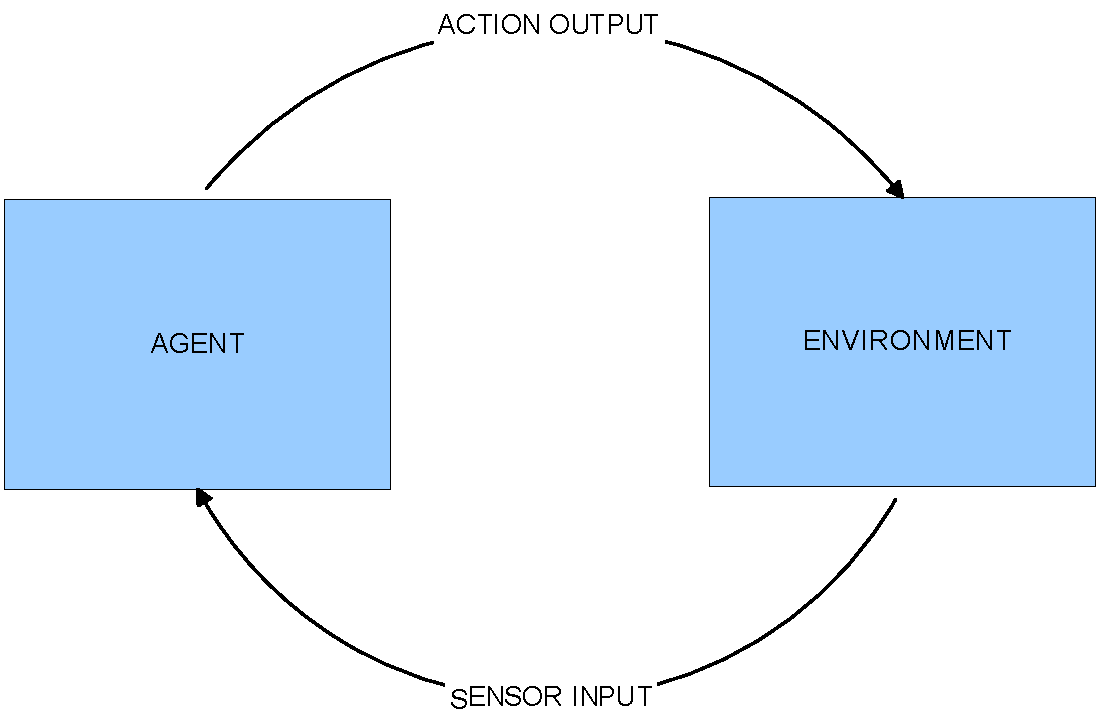
\includegraphics[width=0.8\textwidth]{loop} 
    \end{center} 
\end{frame} 

\begin{frame}{Agent Control Loop...}
    \begin{block}{Pythonic Version of Wooldridge's Agent Control Loop} 
        \showcode{wooldridge.py} 
    \end{block} 
\end{frame} 

\begin{frame}{Or the BDI Control Loop...}
    \begin{itemize}
        \item Begin to look at the agent control loop and the interaction
              with the environment in more detail.
        \item The interaction between agent and environment needs to be
              broken down into components, step by step.
        \item Start looking at how inputs/outputs are generated...
              i.e. look at sensors and actuators.
    \end{itemize} 
\end{frame} 

\begin{frame}{Let dig deeper...}
Five
\end{frame} 

\begin{frame}{A level down...}
    \begin{center}
        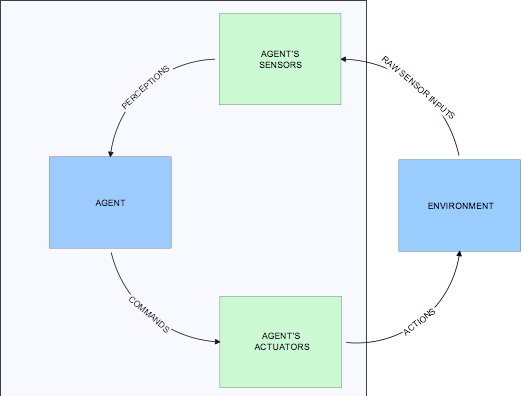
\includegraphics[width=0.7\textwidth]{sensorsactuators} 
    \end{center} 
\end{frame} 

\begin{frame}{Labels in the Environment}  
Seven
\end{frame} 

\begin{frame}{We can begin to formulate a theory...}
Eight
\end{frame} 

\begin{frame}{Agent Mental States}
Nine
\end{frame} 

\begin{frame}{Agent Mental State in the Loop...}
Ten
\end{frame} 

\begin{frame}{Perception and Mental State}
Eleven
\end{frame} 

\begin{frame}{The Agent-Environment Loop Revisited}
Twelve
\end{frame} 

\begin{frame}{Intention Based Feedback Loop}
Thirteen
\end{frame} 

\begin{frame}{Environmental Representation} 
Fourteen
\end{frame} 

\begin{frame}{So what is the goal then?}
Fifteen
\end{frame} 

\begin{frame}{Affordances}
Sixteen
\end{frame} 

\begin{frame}{Example: Jumping a Creek} 
Seventeen
\end{frame} 

\begin{frame}{How do we build such an agent?}
Eighteen
\end{frame} 

\begin{frame}{Issues (1)}
Nineteen
\end{frame} 

\begin{frame}{Issues (2)}
Twenty
\end{frame} 

\begin{frame}{Example} 
Twenty One
\end{frame} 

\end{document}
